\documentclass{../lab}
\usepackage[section]{placeins}
\labacronym{GMA}
\labtitle{Gamma Ray Spectroscopy}

\begin{document}

\maketitle

\tableofcontents

\vspace{1em}

\href{http://experimentationlab.berkeley.edu/sites/default/files/images/DetectorCalibration.pdf}{\textbf{DetectorCalibration.pdf}}

\section{Gamma Ray Description (GMA)}

\begin{enumerate}
    \item \textbf{Note that there is NO eating or drinking in the 111-Lab anywhere, except in rooms 282 \& 286 LeConte on the bench with the BLUE stripe around it.} Thank You the Staff.
\end{enumerate}

The purpose of this experiment is to study some properties of the gamma ray. First, this lab will walk you through some tests to show you how the equipment is affected by your settings. You will then use the gamma rays from some known sources to calibrate your detector, and verify the inverse-square law. Finally, you will make some measurements that will allow you to calculate the mass attenuation coefficients for several materials at several energies.

The experiment offers a good acquaintance with a number of important devices, including a pulse height analyzer, scintillator and photomultiplier tube (PMT). It is well suited for data analysis with a computer.

The gamma rays enter a NaI(Tl) scintillator crystal, which converts them into many lower-energy photons. These photons travel through the crystal to the photocathode of a photomultiplier tube, where they are converted into electrons by means of the photoelectric effect. The photoelectrons are sent through a series of electrodes where the number of electrons is multiplied. At the anode, a pulse of current is produced.

The number of lower energy photons produced in the scintillator is proportional to the deposited energy of the incident gamma ray, and the number of electrons produced is proportional to the number of photons incident on the photocathode. Therefore, the pulse height of the signal from the photomultiplier tube is proportional to the energy of the incident gamma ray. A pulse height analyzer is used to display the spectrum of pulses from the photomultiplier tube.

\begin{enumerate}
    \item Pre-requisites: None

    \item Days Allotted for the Experiment: 6

\end{enumerate}

\textbf{All pages in this lab. Note To print Full Lab Write-up click on each link below and print separately}

I. Gamma-ray Spectroscopy

This lab will be graded 20\% on theory, 40\% on technique, and 40\% on analysis. For more information, see the \href{\AdvancedLabSyllabus}{\textbf{Advanced Lab Syllabus}}.

Comments: E-mail \href{\MailDonOrlando}{\textbf{Don Orlando}}

\section{Gamma-Ray Spectroscopy Photos}
\begin{figure}[H]
\captionsetup{justification=centering}
\minipage[t]{0.33\textwidth}
  \href{http://experimentationlab.berkeley.edu/sites/default/files/images/Gma_t1.jpg}{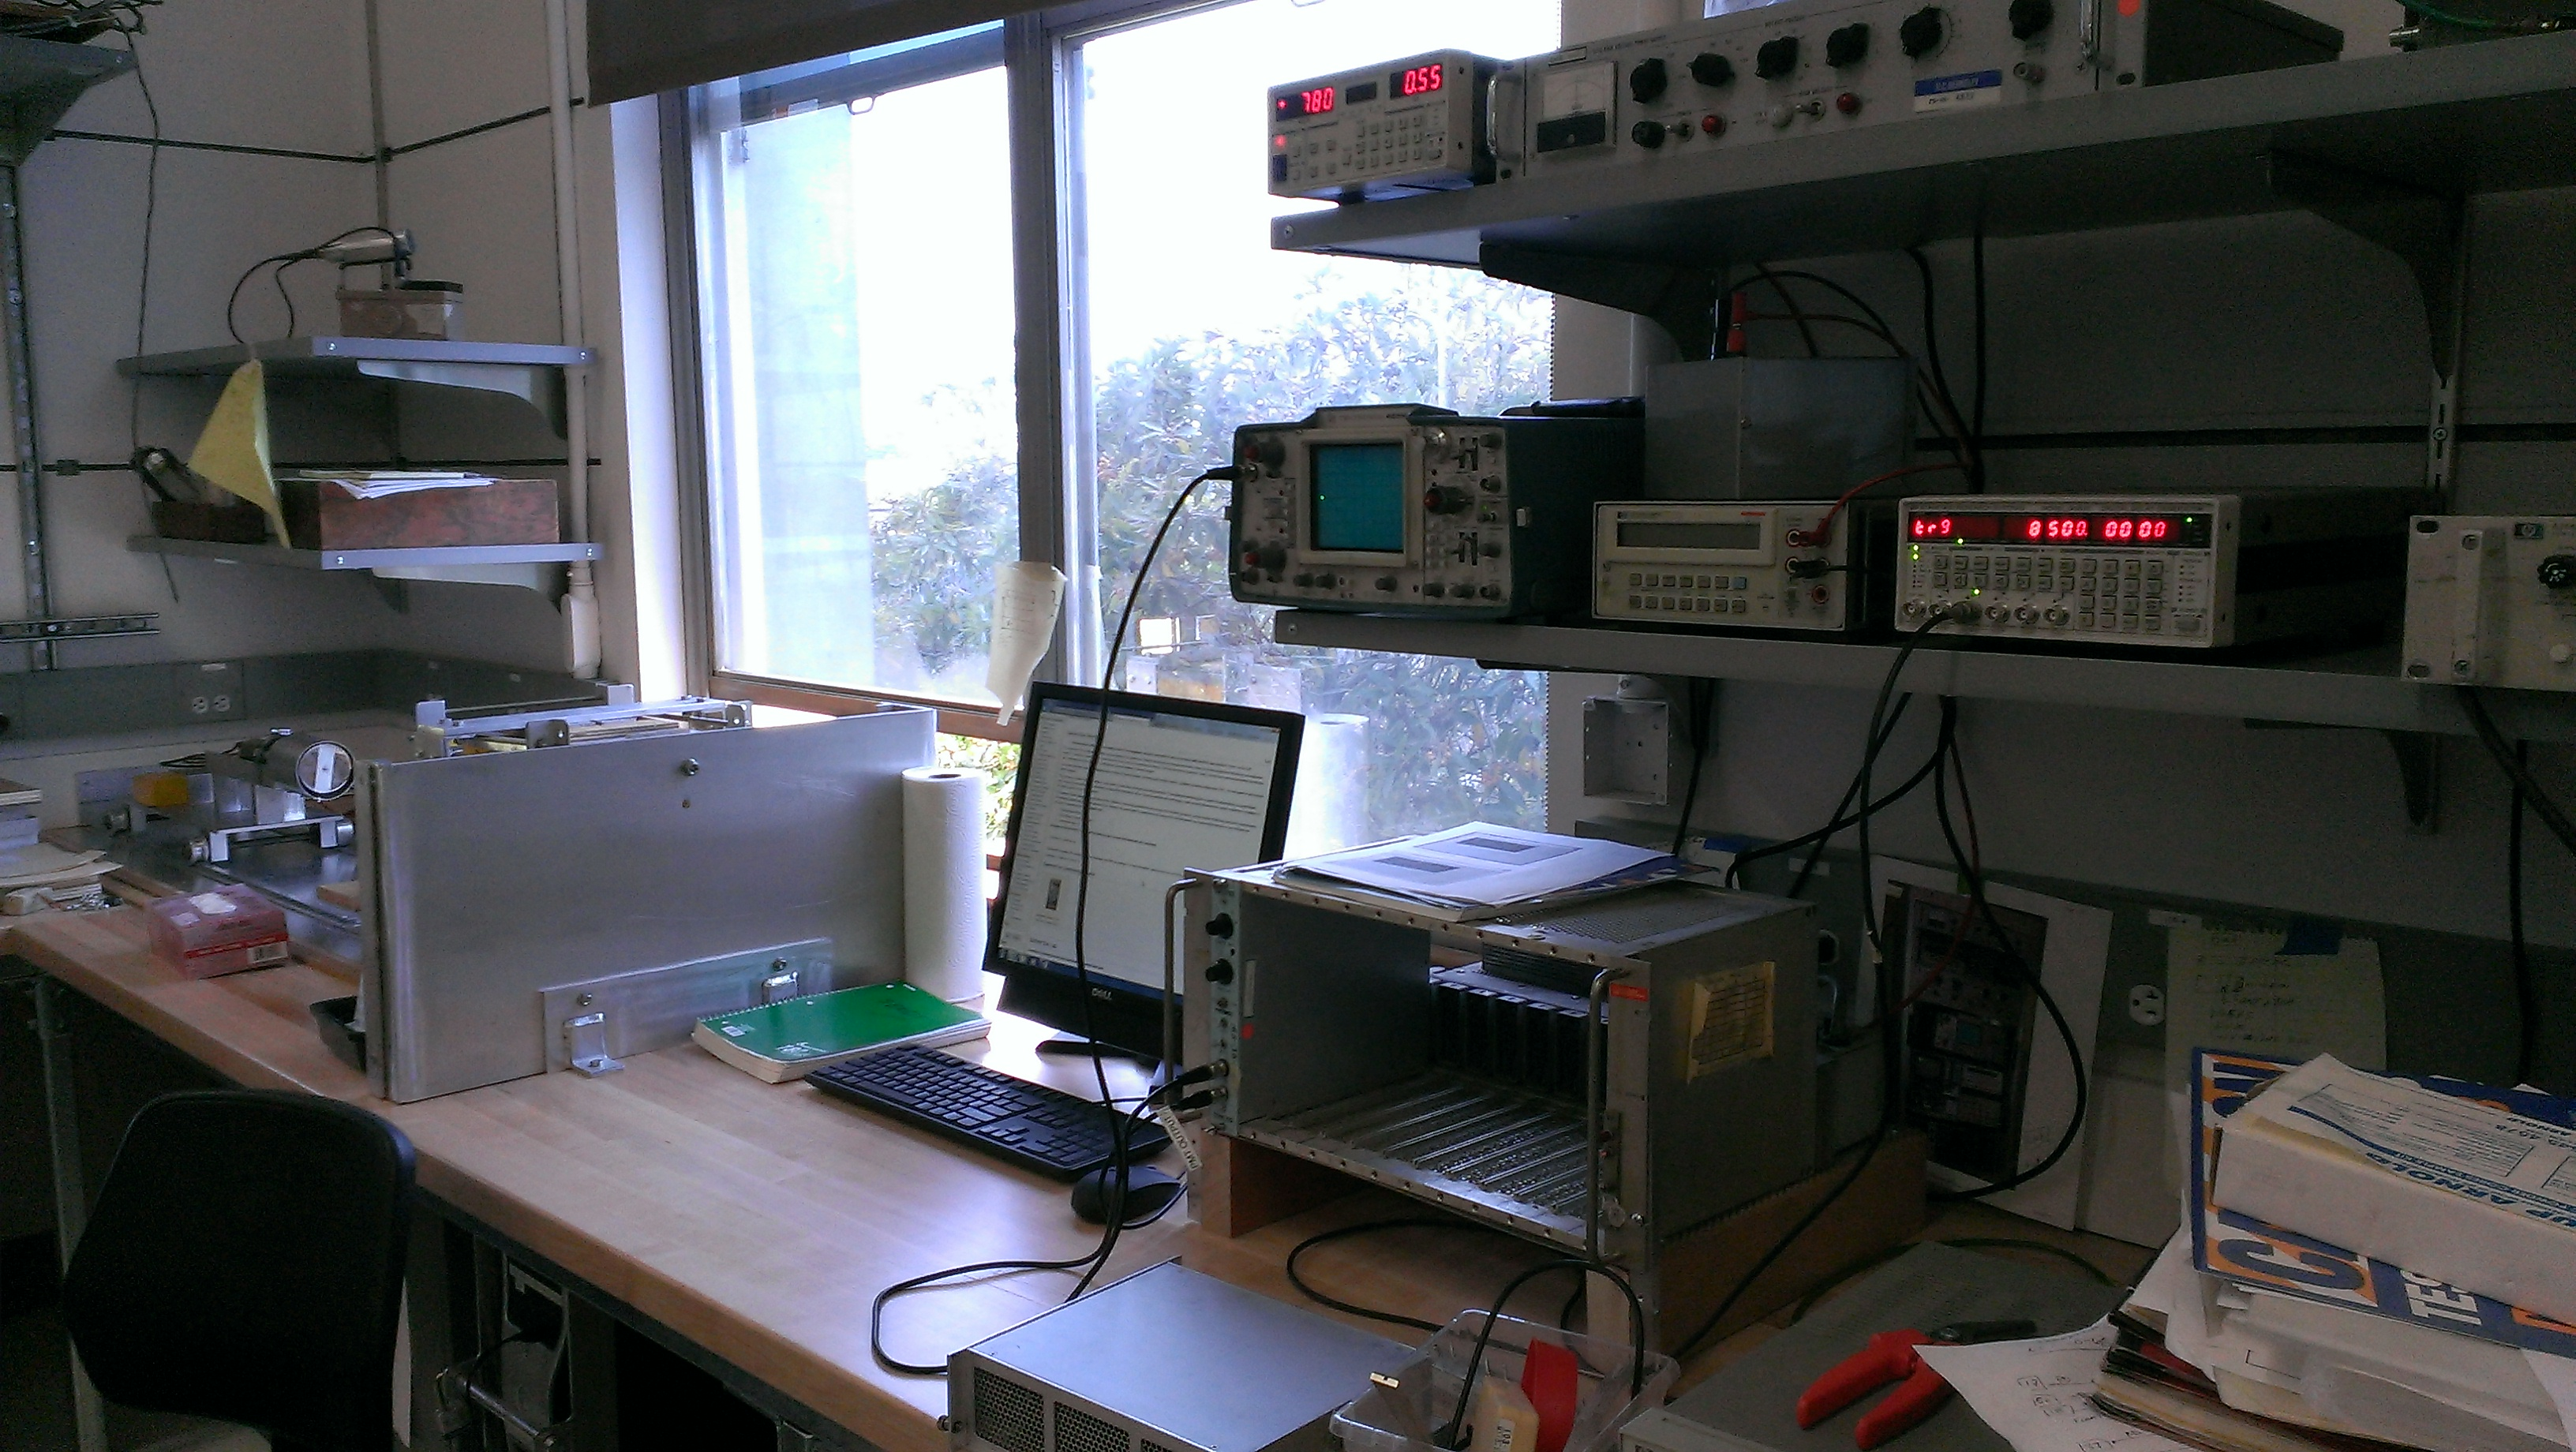
\includegraphics[width=\linewidth,keepaspectratio]{images/Gma_t1.jpg}}
  \caption{Gamma Ray Apparatus \\ \href{http://experimentationlab.berkeley.edu/sites/default/files/images/Gma_t1.jpg}{Click here to see larger picture}}
  \label{fig:Apparatus}
\endminipage\hfill
\minipage[t]{0.33\textwidth}
  \href{http://experimentationlab.berkeley.edu/sites/default/files/images/GMA_Pig_3536-Lg.jpg}{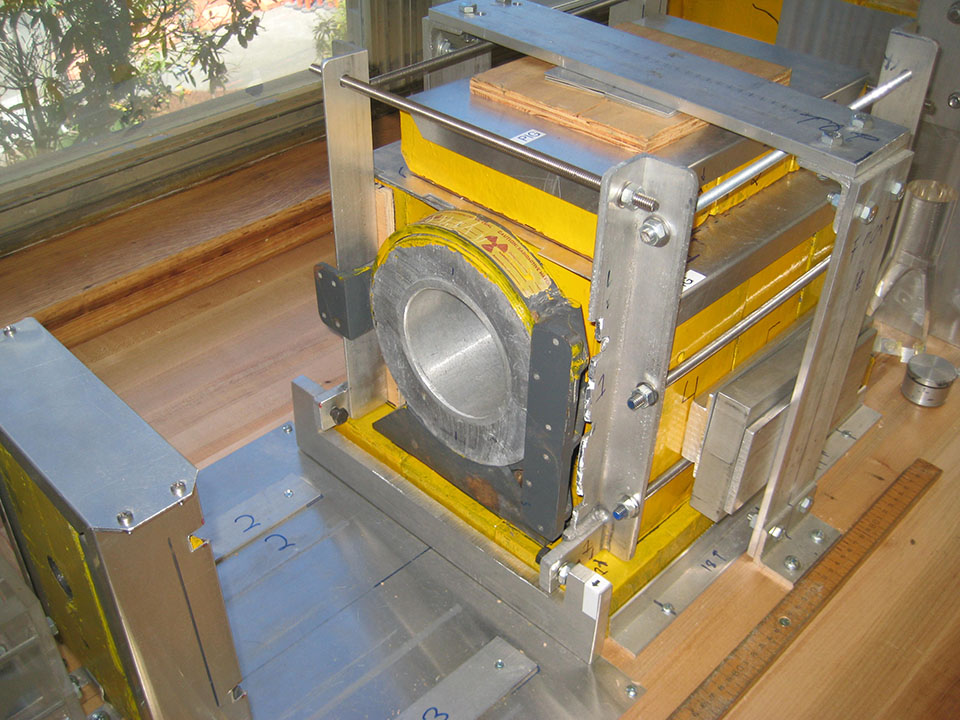
\includegraphics[width=\linewidth,keepaspectratio]{images/GMA_Pig_3536-Lg.jpg}}
  \caption{Lead Pig where source is placed \\
  \href{http://experimentationlab.berkeley.edu/sites/default/files/images/GMA_Pig_3536-Lg.jpg}{Click here to see larger picture}}
  \label{fig:LeadPig}
\endminipage\hfill
\minipage[t]{0.33\textwidth}
  \href{http://experimentationlab.berkeley.edu/sites/default/files/images/GMA_Layout_3537-Lg.jpg}{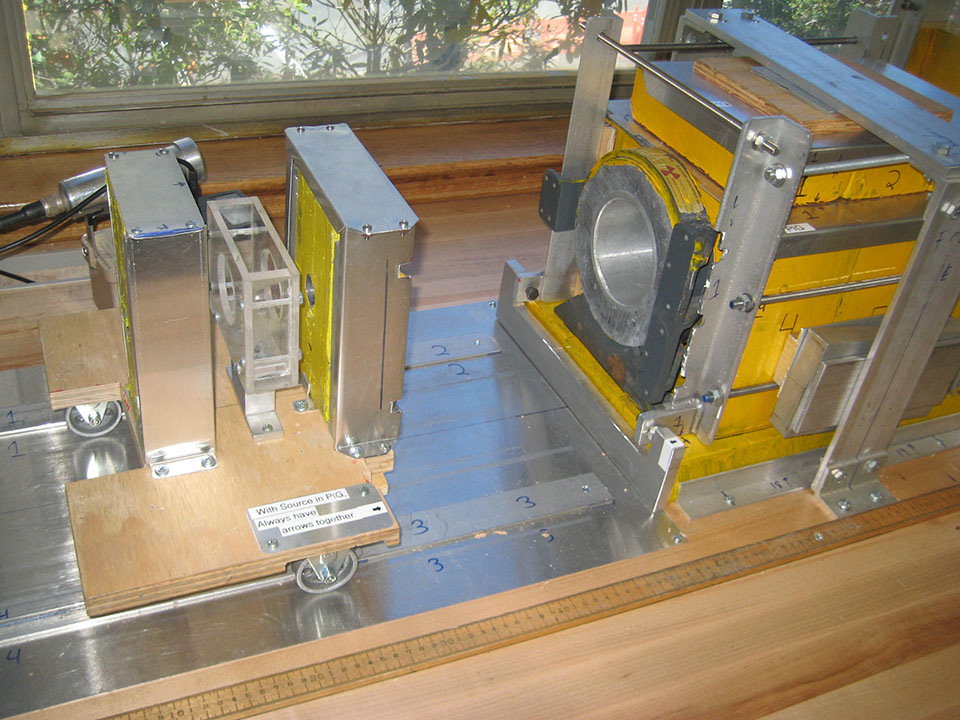
\includegraphics[width=\linewidth,keepaspectratio]{images/GMA_Layout_3537-Lg.jpg}}
  \caption{Pig \& Collimator where source is placed \\ \href{http://experimentationlab.berkeley.edu/sites/default/files/images/GMA_Layout_3537-Lg.jpg}{Click here to see larger picture}}\label{fig:PigCollimator}
\endminipage
\end{figure}

\begin{figure}[H]
\captionsetup{justification=centering}
\minipage[t]{0.33\textwidth}
  \href{http://experimentationlab.berkeley.edu/sites/default/files/images/GMA_Layout_3538-Lg.jpg}{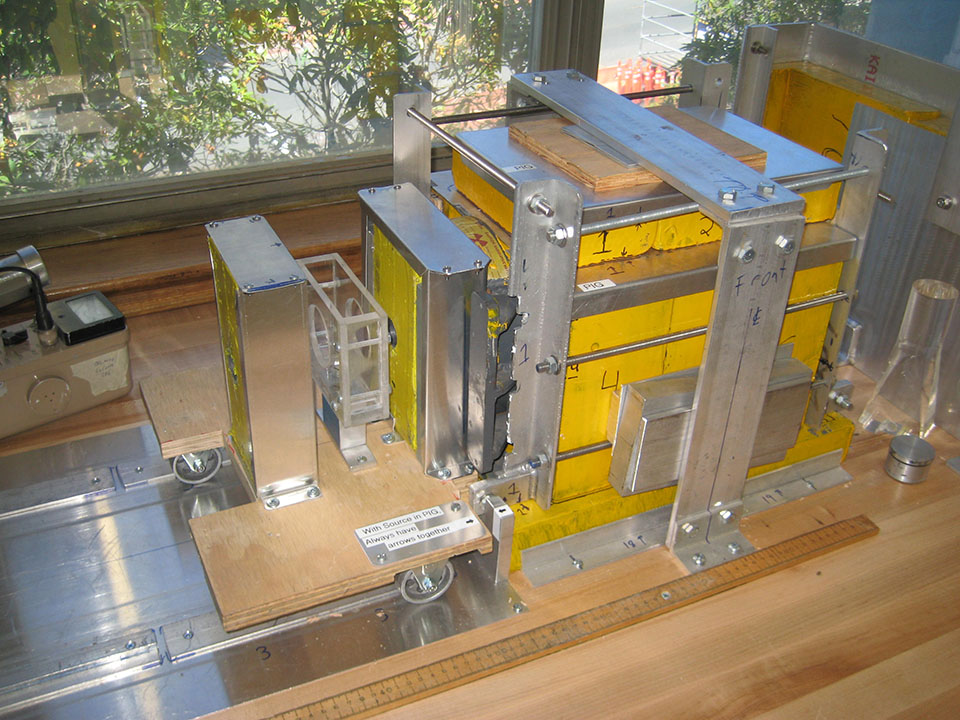
\includegraphics[width=\linewidth,keepaspectratio]{images/GMA_Layout_3538-Lg.jpg}}
  \caption{Collimator moved in place \\ \href{http://experimentationlab.berkeley.edu/sites/default/files/images/GMA_Layout_3538-Lg.jpg}{Click here to see larger picture}}
  \label{fig:CollimatorMovedIn}
\endminipage\hfill
\minipage[t]{0.33\textwidth}
  \href{http://experimentationlab.berkeley.edu/sites/default/files/images/GMA_PMT_3519-Lg.jpg}{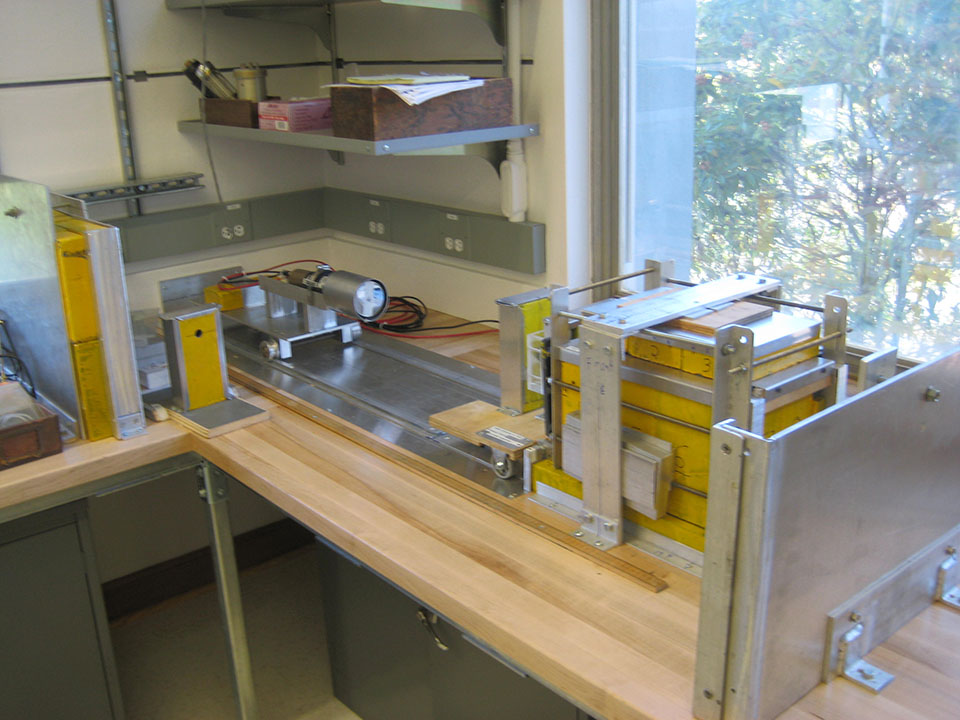
\includegraphics[width=\linewidth,keepaspectratio]{images/GMA_PMT_3519-Lg.jpg}}
  \caption{PMT on Cart \& source Lead Pig Setup \\
  \href{http://experimentationlab.berkeley.edu/sites/default/files/images/GMA_PMT_3519-Lg.jpg}{Click here to see larger picture}}
  \label{fig:PMT}
\endminipage\hfill
\minipage[t]{0.33\textwidth}
  \href{http://experimentationlab.berkeley.edu/sites/default/files/images/GMA_Equip_3518-Lg.jpg}{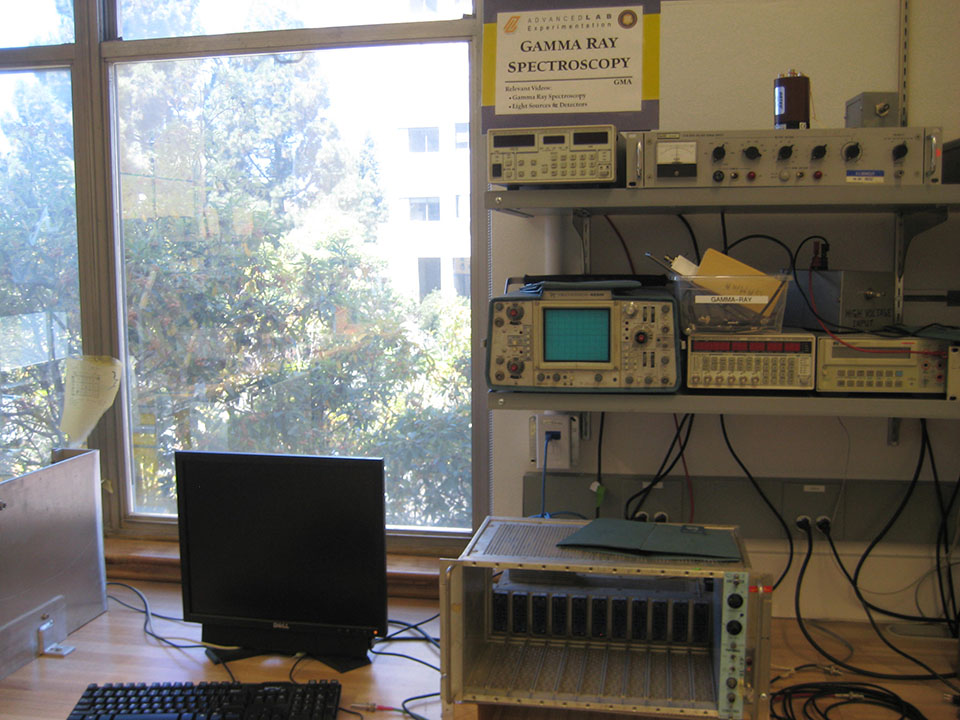
\includegraphics[width=\linewidth,keepaspectratio]{images/GMA_Equip_3518-Lg.jpg}}
  \caption{Gamma Ray Equipment \\ \href{http://experimentationlab.berkeley.edu/sites/default/files/images/GMA_Equip_3518-Lg.jpg}{Click here to see larger picture}}\label{fig:Equipment}
\endminipage
\end{figure}

\begin{figure}[H]
\captionsetup{justification=centering}
\minipage[t]{0.33\textwidth}
  \href{http://experimentationlab.berkeley.edu/sites/default/files/images/GMAimagegeigercounter.jpg}{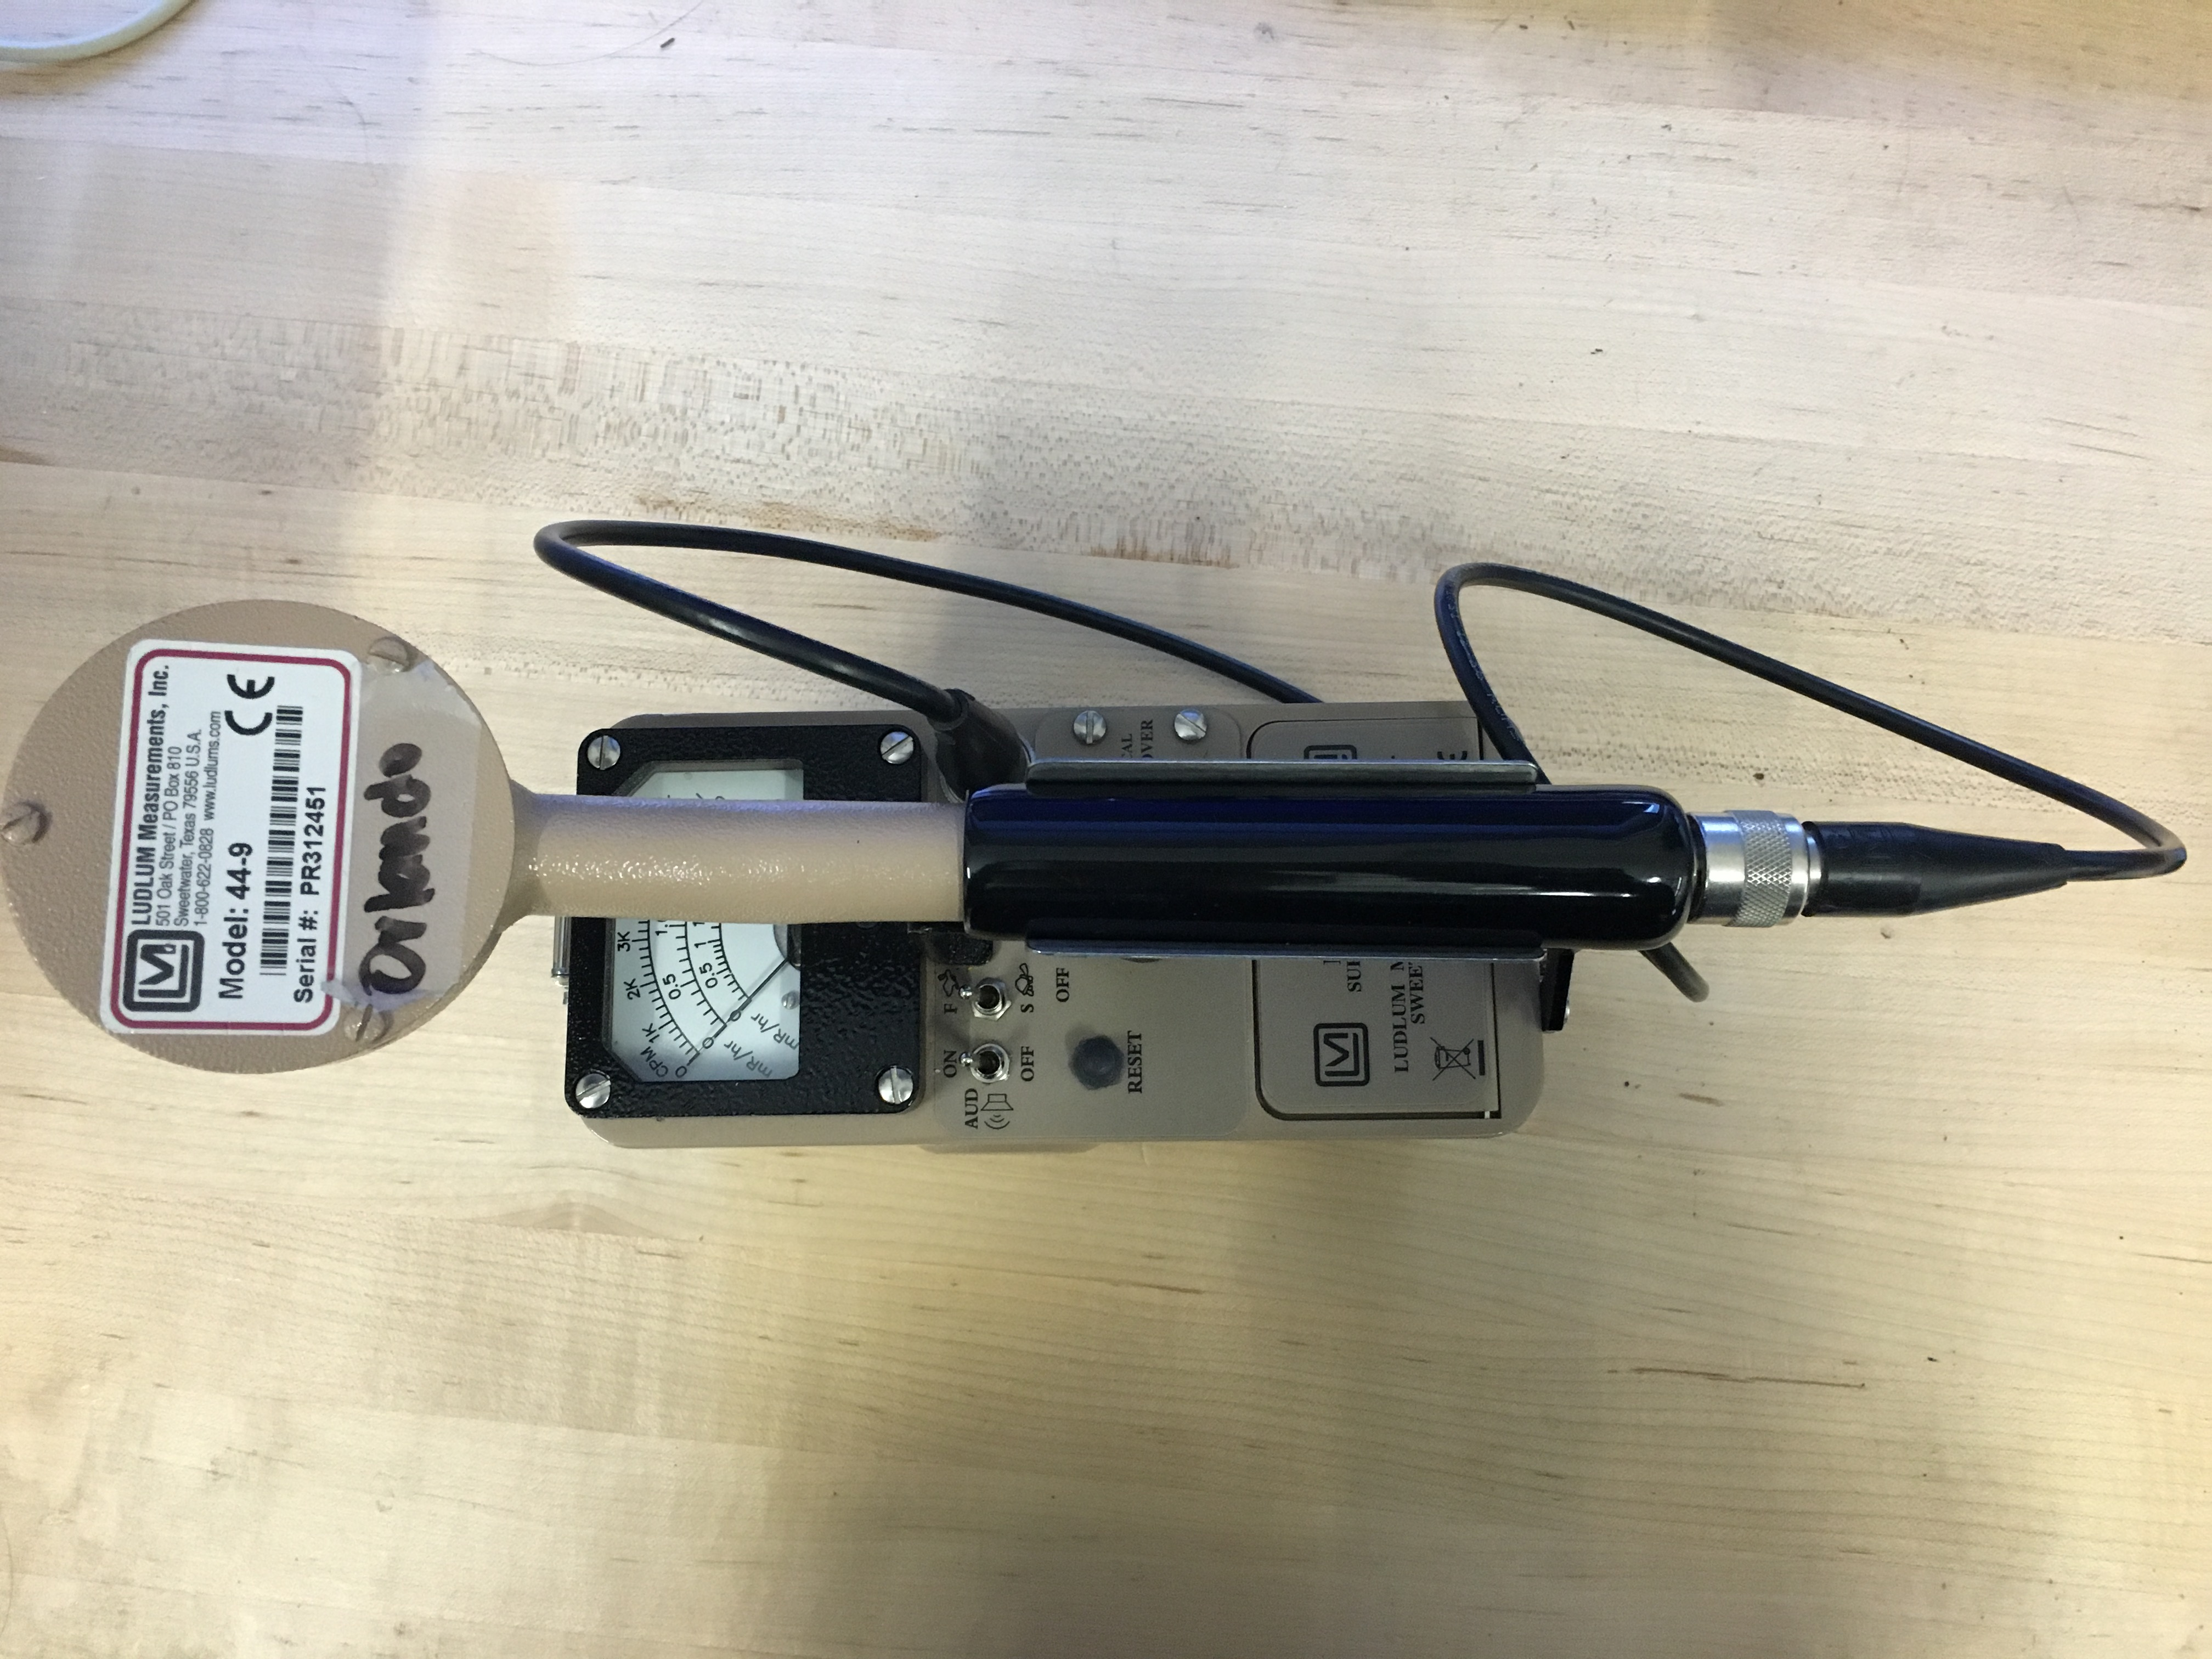
\includegraphics[width=\linewidth,keepaspectratio]{images/GMAimagegeigercounter.jpg}}
  \caption{The Geiger Counter \\ \href{http://experimentationlab.berkeley.edu/sites/default/files/images/GMAimagegeigercounter.jpg}{Click here to see larger picture}}
  \label{fig:GMAgeiger}
\endminipage\hfill
\minipage[t]{0.33\textwidth}
  \href{http://experimentationlab.berkeley.edu/sites/default/files/images/GMAimage_Base_and_PMT.png}{\includegraphics[width=\linewidth,keepaspectratio]{images/GMAimage_Base_and_PMT.png}}
  \caption{Photomultiplier tube and its base\\
  \href{http://experimentationlab.berkeley.edu/sites/default/files/images/GMAimage_Base_and_PMT.png}{Click here to see larger picture}}
  \label{fig:PMTandBase}
\endminipage\hfill
\minipage[t]{0.33\textwidth}
  
\includegraphics[width=\linewidth,keepaspectratio]{images/empty.png}
\endminipage
\end{figure}

\section{Before the 1st Day of Lab and Standard Operating Procedures for the Gamma-Ray Experiment}

\signatures \hyperlink{Variable High-Voltage Supply}{1} \hyperlink{Change of Pulses}{2} \hyperlink{Parameters}{3} \hyperlink{Back-Scatter and Compton Edge Signals}{4} \hyperlink{Intensity Formula}{5} 

\begin{enumerate}
    \item \emph{\textbf{Note: In order to view the private Youtube videos hosted by the university, you must be signed into your berkeley.edu Google account.}} \\
    View the \href{http://youtu.be/cZGMngx-6yE}{\textbf{Gamma Ray Video}}. The equipment for this lab has changed over the years making the last part of the video inconsistent with the procedure on this lab but it is nonetheless useful for understanding how the set-up works.

    \item View the \href{http://youtu.be/KHxtzF5pZZM}{\textbf{\textbf{Radiation Safety Video}}} After watching the video in the 111-Lab, get a pink Radiation Safety form from a 111-Lab staff person. Fill it out \& sign the form for getting a \textbf{Radiation Ring}.

    \item Now complete the Radiation Safety Training \href{http://experimentationlab.berkeley.edu/RadiationSafety}{\textbf{Radiation\_Safety}} \textbf{After completion of Training turn in all forms to Don Orlando.}

    \item \signatures \hyperlink{Variable High Voltage Supply}{ 1}  \hyperlink{Change of Pulses}{ 2} \hyperlink{Parameters}{ 3} \hyperlink{Back-Scatter and Compton Edge Signals}{ 4} \hyperlink{Intensity Formula}{ 5}

    \item View the \href{http://youtu.be/jR54387Wd6c}{\textbf{Introduction to Error Analysis video}} and \href{http://experimentationlab.berkeley.edu/EAX}{\textbf{\textbf{Error Analysis Notes}}}.

    \item Also view \href{http://youtu.be/lQKLakISoBA}{\textbf{Light Sources and Detectors}} video.

    \item Read the Standard Operating Procedures (SOP) for this lab before starting \href{http://experimentationlab.berkeley.edu/sites/default/files/images/SOP\_3271\_Cs-137\_Na-22\_Co-60\_Mn-54\_Am-241\_Fe-55\_2014.pdf}{\textbf{SOP\_3271\_Cs-137\_Na-22\_Co-60\_Mn-54\_Am-241\_Fe-55\_2014}}.

    \item Last day of the experiment please fill out the \href{\ExperimentEvaluation}{\textbf{Experiment Evaluation}}

\end{enumerate}

\noindent\textbf{Suggested Reading:}

\begin{enumerate}
    \item Knoll, \emph{Radiation Detection and Measurement}, John Wiley and Sons, New York (1979):
    \begin{enumerate}
        \item \href{http://physics111.lib.berkeley.edu/Physics111/Reprints/GMA/01-Radiation\_Detection\_and\_Measurement\_CH\_01.pdf}{\textbf{Ch. 1}} \S IV pp 16-25 (Information about the sources of EM radiation),
        
        \item \href{http://physics111.lib.berkeley.edu/Physics111/Reprints/GMA/01-Radiation\_Detection\_and\_Measurement\_CH\_02.pdf}{\textbf{Ch. 2}} \S III pp 62-71 (How gamma rays interact),
        
        \item \href{http://physics111.lib.berkeley.edu/Physics111/Reprints/GMA/01-Radiation\_Detection\_and\_Measurement\_CH\_03.pdf}{\textbf{Ch. 3}} \S I-VI pp 79-95 (Detectors in general)
        
        \item \href{http://physics111.lib.berkeley.edu/Physics111/Reprints/GMA/01-Radiation\_Detection\_and\_Measurement\_CH\_09.pdf}{\textbf{Ch. 9}} \S I - \S III pp 272-284 (Photomultiplier tubes)
        
        \item \href{http://physics111.lib.berkeley.edu/Physics111/Reprints/GMA/01-Radiation\_Detection\_and\_Measurement\_CH\_10.pdf}{\textbf{Ch. 10}} \S I-IV(B) pp 306-338 (Scintillators).
    \end{enumerate}
    
    \item 

    \item Harshaw Scintillation Phosphors; \href{http://physics111.lib.berkeley.edu/Physics111/Reprints/GMA/Harshaw\%20scintillation\%20phosphors.pdf}{\textbf{Harshaw Scintillators}} and \href{http://experimentationlab.berkeley.edu/sites/default/files/pdfs/Nal\_Crystal\_Information.pdf}{\textbf{NaI Crystal Information}}
    
    \item \href{http://physics111.lib.berkeley.edu/Physics111/Reprints/GMA/RCA\%20PMT.pdf}{\textbf{RCA Photomultiplier Tube Manual}}
    
\end{enumerate}

\noindent More \hyperref[sec:References]{References}

[\href{\LabReprints}{\textbf{Physics 111 Library Site}}]

You should keep a laboratory notebook. The notebook should contain a detailed record of everything that was done and how/why it was done, as well as all of the data and analysis, also with plenty of how/why entries. This will aid you when you write your report.

\section{Objectives}

\begin{itemize}
    \item Learn what real experimental physics is about

    \item Learn the synergy between experimental and theoretical work

    \item Learn to use pieces of equipment that are commonly used in research

    \item Learn how measurements are performed, analyzed, and interpreted.

    \item Learn how to present your work and results

    \item Learn problem solving strategies

    \item Learn how to manage and organize your time

    \item Learn about gamma ray spectroscopy using doped sodium iodide scintillator

    \item Thorough understanding on how the photo multiplier (PMT) works, and how it is used with the CANBERRA amplifier.

    \item You should also gain a well-developed understanding on how the pulse height analyzer works.

    \begin{itemize}
        \item Formation of the peaks on the spectrum

        \item Identify sources that cause the peaks to spread wider.

        \item Learn how to calibrate the PHA.

    \end{itemize}

    \item Measure the spectra of various radioactive sources.

    \item Verify the inverse square law for radiation.

    \item Determine the absolute intensity of the $^{137}$Cs source.

    \item Determine the mass attenuation coefficients of several materials at several energies.

    \item Learn how to operate the Digital Delay Operator.

\end{itemize}

\section{Introduction}

The measurement of energy levels of atomic, molecular, and nuclear systems constitutes a large part of experimental physics. This experiment examines gamma rays, which come from transitions between nuclear energy levels, with emphasis on their interaction with matter. This experiment is a little different from most in the 111 Laboratory in that a lot of what you do will be oriented towards learning about the equipment and its capabilities, rather than striving to achieve some experimental result. It is important that before you start to use the tools understand their purpose in this lab. Stop and think about what it is that you're trying to accomplish by using this tool, this can save you a great amount of valuable time.

\section{Apparatus}

\begin{enumerate}
    \item \href{http://physics111.lib.berkeley.edu/Physics111/Reprints/GMA/905-series-nai-radiation-detectors.pdf}{\textbf{PMT}} (\href{http://experimentationlab.berkeley.edu/sites/default/files/images/905-4.pdf}{\textbf{905-4}}) with \href{http://physics111.lib.berkeley.edu/Physics111/Reprints/GMA/266-Photomultiplier-Base.pdf}{\textbf{Ortec 266}} Base
    
    \item Stanford Research Systems  \href{http://physics111.lib.berkeley.edu/Physics111/Equipment_Manuals/GMA/PS325m.pdf}{\textbf{PS325}} High Voltage Power Supply

    \item Canberra Amplifier  \href{http://physics111.lib.berkeley.edu/Physics111/Reprints/GMA/GMA\%20OCR\%20Canberra\%20spectroscopy\%20amp\%20816.pdf}{\textbf{816}}

    \item Stanford Research Systems  \href{http://physics111.lib.berkeley.edu/Physics111/Equipment_Manuals/GMA/DG645m.pdf}{\textbf{DG645}} Digital Delay Generator

    \item National Instruments \href{http://physics111.lib.berkeley.edu/Physics111/Reprints/GMA/NI_PCI-5124.pdf}{\textbf{NI-5124 Digitizer Card}} (Used for digital Soft Scope and Pulse Height Analyzer)

    \item Oscilloscope

\end{enumerate}

\subsection{Safety}

\textbf{Remember the Lead Bricks are heavy, at least 30 to 50 pounds each. If it is knocked off the bench and falls onto someone's foot it will smash it to pieces.}

You must wear a radiation ring when you are working with the gamma-ray apparatus. You should also always wear vinyl gloves when handling the radioactive sources, but remove and \textbf{discard} them when adjusting the equipment or you will defeat the purpose. The sources are located in a lead container, and this should be kept closed. Keep the sources in their plastic bags. When you use the sources, put the clamps on the bags, not on the source itself inside the bag. Any rupture of the source package will cause leakage of radioactive materials - very low-level radiation and not a serious health hazard, yet it will require discarding the source and a decontamination of the bench area or wherever the source has been.

Do not stack the lead bricks on the lab bench - it would be very dangerous to do so. They are quite heavy and the kinetic energy they would gain from a one-meter fall is more than that enough to shatter a human toe (we know this from direct experience). In addition, you will find experimentally that some of the gamma rays can Compton scatter off these bricks and contribute to the scattering portion of your spectra.


\textbf{Gloves:}
\begin{enumerate}
    \item Wear a pair of nitrile gloves before you touching any radioactive sample or any container that has radioactive sources inside.
    
    \item Dispose the contaminated gloves into the specified bin under the desk.
    
    \item To prevent any potential contamination from leakage, do not wear gloves while touching any experimental device, such as the high voltage power source, the oscilloscope, the lab computer mouse or the keyboard once you have already touch the radioactive sample.
\end{enumerate}

\textbf{Geiger Counter:}
\begin{enumerate}
    \item At the end of each experiment day, use the Geiger counter (See Figure~\ref{fig:GMAgeiger}) to check the radioactive level around the area of GMA experiment as well as your body.
    
    \item Report any suspiciously hihg intensity of radiation to a GSI, Professor, or Donald Orlando as soon as possible.
\end{enumerate}

\subsection{Radioactive sources}

The radioactive sources are in plastic bottles with the radioactive material embedded in epoxy. The original activity and date are on the label of the bottle. The sources emit radiation in all directions. To use a source, hang the bottle by grasping its top with a clamp so that the source is at the same height as the center of the detector.

The following are the radioactive sources used in this experiment.

\begin{center}
    \begin{tabular}{l|l|l}
        Source     & Energy (MeV) & Half-life \\\hline
        $^{22}$Na  &  0.511, 1.28 & 2.6 years \\\hline
        $^{137}$Cs &  0.6616      & 30 years  \\\hline
        $^{60}$Co  &  1.17, 1.33  & 5.2 years \\\hline
        $^{54}$Mn  &  0.84        & 312 days
    \end{tabular}
\end{center}

\subsection{Detection}
The gamma rays in this experiment are detected with a thallium-doped sodium iodide [NaI(Tl)] crystal (3.0`` in diameter and 3'' in height: verify these dimensions) mounted on a PMT (See Ortec Specs \href{http://physics111.lib.berkeley.edu/Physics111/Reprints/GMA/905-series-nai-radiation-detectors.pdf}{\textbf{905-4}} Model: 2.00 @ 0.5 MeV and 1.30 @ 2.0 MeV; 3M3/3X with tube base \href{http://physics111.lib.berkeley.edu/Physics111/Reprints/GMA/266-Photomultiplier-Base.pdf}{\textbf{Ortec \# 266}}). \textbf{The maximum voltage supplied to the PMT is +800 Volt DC}. This crystal emits photons in the visible range when struck by gamma rays, and is hence called a ``scintillating'' crystal. These visible photons are detected and amplified by the photomultiplier tube (PMT), which consists of a photocathode, a focusing electrode, and 10 or more dynodes that multiply the number of electrons striking at each dynode. The PMT then outputs a pulse of electrical current with an amplitude proportional to the energy of the incident gamma ray. This pulse is further amplified with an external amplifier and then fed into a NI-5124 Pulse Height Analyzer. A chain of resistors typically located in a plug-in tube base assembly biases the anode and dynodes. Complete assemblies including the scintillator and PMT are available. 

The Pulse Height Analyzer (PHA) is a LabView program, \textbf{``PHA-5124.exe''}, using the National Instruments NI-5124 Digitizer Card. National Instruments donated this card to us for the Physics 111-Lab. You first check the signals out of the pre-amplifier with the \textbf{Soft Scope program} using the \href{http://physics111.lib.berkeley.edu/Physics111/Reprints/GMA/NI_PCI-5124.pdf}{\textbf{NI-5124}} Card. Pulses of varying amplitudes between 0 and 8 volts are sampled into 1024 increments (or what you select in program control Tab). When a pulse representing a detected gamma ray is received, the PHA-5124 determines its amplitude and puts it into the correct channel (bin). Because the amplitude expressed as a voltage is proportional to the energy of the incoming gamma ray (a fact you should explain in your report), the accumulated counts form a distribution called an energy spectrum on the screen - the number of gamma rays that have been detected in each energy bin.

\checkpoint{Variable High Voltage Supply}{What is the role of the variable high voltage and how does it affect the output amplitude on the oscilloscope?}

\section{Procedure}

\begin{enumerate}
    \item Before turning on the SRS High Voltage Power Supply, you need to make sure that the polarity is set to positive, and that the High Voltage line is connected to the PMT (this should already be the case). The polarity may be set using a flat-head screw-driver on the back of the unit. The groove aligns with the chosen setting, and should already point to positive. There should be a red BNC cable running from the back of the power supply to the \textbf{POS HV} input at the PMT base. Before powering on the power supply, make sure that the black High Voltage switch is set to \textbf{OFF/RESET}. Now, power on the power supply. You first need to set the power supply to provide 780V. The word \textbf{SET} should be backlit by a green LED, allowing you to adjust the power supply potential. Above it, the smallest LED screen should read 780 (V). If it does not, type 780 and click \textbf{ENTER}. Once set, this will be our starting point. If you are sure that everything is connected properly, turn on the High Voltage using the \textbf{High Voltage} switch. The word \textbf{ON} should now be back-lit with a red LED. To have stable operation, it is better to leave the high-voltage power supply running during the period that you sign up for the experiment. Remember that a High Voltage supply such as this one may need up to 15 min of warm-up time before the potential stabilizes, therefore it is a good idea to let it run for some time before taking data. If there is a problem with this power supply, alert the staff. There is an older HV power supply available (Fluke 415B) if necessary.
    
    \begin{figure}[h]
        \centering
        \href{http://experimentationlab.berkeley.edu/sites/default/files/images/250px-HV-SRS-PSU.jpg}{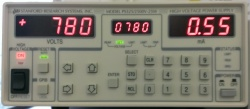
\includegraphics[width=0.6\linewidth]{images/250px-HV-SRS-PSU.jpg}}
        \caption{SRS Power Supply}
        \label{fig:250px-HV-SRS-PSU}
    \end{figure}

    Place the $^{137}$Cs source into the Circular Lead Pig \href{http://experimentationlab.berkeley.edu/sites/default/files/images/GMA_Pig_3536-Lg.jpg}{\textbf{See picture Figure~\ref{fig:LeadPig} above.}} 20 to 25 cm away from the detector with lead colliminator in front of the source. Make sure that the collimator assembly is in place as shown \href{http://experimentationlab.berkeley.edu/sites/default/files/images/GMA_Layout_3537-Lg.jpg}{\textbf{See picture Figure~\ref{fig:PigCollimator}}} \href{http://experimentationlab.berkeley.edu/sites/default/files/images/GMA_Layout_3538-Lg.jpg}{\textbf{\& Figure~\ref{fig:CollimatorMovedIn} above.}} Look at the output of the PMT on a fast scope (Tektronix type), then look at it with the ``Soft Scope program using the Digitizer NI-5124. To match impedance, use a 50-ohm terminator on a BNC ''tee" going into the scope. Look for a faint signal about 0.5 $\mu$sec wide and -50 mV high (see Figure~\ref{fig:250px-GMAimage003}). You'll have to play with the triggering to get this, and you'll probably have to turn up the trace intensity and shield the screen from glare. Each trace of this signal is the electron pulse coming from the PMT that represents a gamma ray striking the detector. The signal is blurred because of many negative pulses with different amplitudes coming from the PMT.

    \begin{figure}[h]
        \centering
        \href{http://experimentationlab.berkeley.edu/sites/default/files/images/250px-GMAimage003.gif}{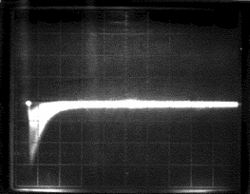
\includegraphics[width=0.5\linewidth]{images/250px-GMAimage003.png}}
        \caption{Scope picture of trace: PMT Output, $^{137}$Cs Source Scope: 50 mV/div; 0.5 $\mu$sec/div.}
        \label{fig:250px-GMAimage003}
    \end{figure}

    \item The CANBERRA AMPLIFIER (amp), \href{http://experimentationlab.berkeley.edu/sites/default/files/images/GMA_Equip_3518-Lg.jpg}{\textbf{located in the equipment rack Figure~\ref{fig:Equipment} above}}, amplifies the small pulses from the PMT to a sufficiently large one necessary for the PHA-5124 program. Feed the output of the PMT into the amp (you don't need a terminator here). Set the INPUT switch to NEG (since the PMT output are negative pulses), and the MODE switch to UNI (since the pulses are unipolar - that is, they are entirely negative as opposed to a signal that has positive as well as negative parts). Look at the output of the amp (without a terminator); you should see a positive pulse about 1 $\mu$sec wide followed by a negative pulse that is of no interest (see Figure~\ref{fig:250px-GMAimage004}). Watch the effects of varying the gain controls, it's recommended to start with FINE GAIN at 2.5 and COARSE GAIN AT 4. Set the gain to produce a pulse that does not have a flat top.

    \begin{figure}[h]
        \centering
        \href{http://experimentationlab.berkeley.edu/sites/default/files/images/250px-GMAimage004.gif}{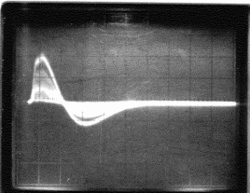
\includegraphics[width=0.5\linewidth]{images/250px-GMAimage004.png}}
        \caption{Amplifier Output Scope: 2 V/div; 1 $\mu$sec/div}
        \label{fig:250px-GMAimage004}
    \end{figure}

    If you have trouble with this unit, there should be a 472A Spectroscopy Amplifier in storage which can perform the same task. You should report the problem of the amplifier to the staff, and they will provide you with a different amplifier.

\end{enumerate}

\section{Pulse Height Analyzer (PHA Digitizer)}

\begin{enumerate}
    \item The \href{http://experimentationlab.berkeley.edu/PHA-5124Program}{\textbf{PHA-5124}} is explained here. For this experiment we use the National Instruments Digitizer Card \href{http://physics111.lib.berkeley.edu/Physics111/Reprints/GMA/NI_PCI-5124.pdf}{\textbf{NI-5124}}.
    \begin{enumerate}
        \item To start, plug the output of the amp into the Digitizer channel 0 located at the rear of the computer (The Digitizer cable should be labeled and connected to a T). Using a \textbf{$^{60}$Co source} you should see a spectrum similar to Figure~\ref{fig:350px-CO-60_Spectrum}.

        \begin{figure}[h]
            \centering
            \href{http://experimentationlab.berkeley.edu/sites/default/files/images/350px-CO-60_Spectrum.png}{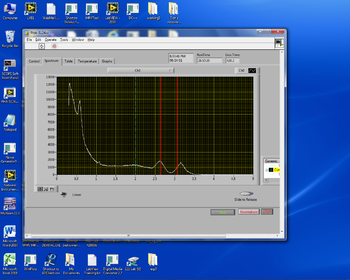
\includegraphics[width=0.5\linewidth]{images/350px-CO-60_Spectrum.png}}
            \caption{PHA display. Counts vs Energy of $^{60}$Co}
            \label{fig:350px-CO-60_Spectrum}
        \end{figure}

    \checkpoint{Width of a peak}{For a given radioactive sample (in a bottle), the emitted gamma rays are mono-energetic. What is the reason that we observe the peaks with finite width in the Pulse Height analyzer instead of delta functions?}
    

        \item The other adjustments you should experiment with are the LLD on the Control Tab in the program: this sets the Lower Level Discriminator so that the PHA will ignore pulses with amplitudes below the setting. This way the system doesn't spend its time with unwanted pulses like low-level noise. To set it properly look at the Soft Scope program display. Setting the LLD too low will allow the program to trigger on noise, and overload the program. Set the LLD at a reasonable level that is above the noise level, but below the level of the physical processes that you are interested in. You may find that you still have some noise causing your spectrum to look distorted and this could be due to a couple of factors. Try thinking about the PMT and what are some of the variables that can contribute to non-linearity in it (this should hint you on what should be adjusted).

        \item After setting the LLD, STOP the unit from acquiring, change your source back to $^{137}$Cs and ACQUIRE again. You should see one peak start to form in the middle of the display, along with a ``mess'' forming to its left. The peak corresponds to the 0.662 MeV $^{137}$Cs gamma rays; what are the peaks to its left? It may be useful to try thinking about what determines the height of the peaks on the graph. Press STOP to stop the accumulation of counts when the peak is reasonably well formed. See Figure~\ref{fig:250px-GMAimage004}.

        \item After collecting a data set and saving it to a file you can use a computer with Matlab or some other program to display the channel number and counts of any channel that you want to see. In this experiment we are only interested in channel 0.

    \end{enumerate}

    \item \textbf{Remember The Maximum Voltage is +800 VDC.} Measure the relative gain of the photomultiplier tube as a function of high voltage using the photopeak of the Cs source. The purpose of this exercise is to gain familiarity with the gain of a photomultiplier. It is not an examination of the non-linearity of the gain curve. To do this, vary the high voltage to the PMT using the knobs on the 3 KV High Voltage power supply only, and watch to see where the Cs peak moves. Because the peak channel number is equivalent to some pulse height, by recording the peak channel number at each voltage we can determine the relative gain as a function of the PMT high voltage. Start at around +400 volts, and stop at about +800 volts (change the high voltage by 10 volts at a time) to determine the relation between gain and high voltage. \textbf{Do not exceed 800V.} Plot the results. Explain the plot, particularly the behavior at the higher (more positive) voltage settings. Then, make another plot to show that the gain is related to the applied high voltage as a power law (see the section on Photomultiplier Tube in Knoll \href{http://physics111.lib.berkeley.edu/Physics111/Reprints/GMA/01-Radiation\_Detection\_and\_Measurement\_CH\_09.pdf}{\textbf{Ch.9}}).

    \item To examine the capabilities and linearity of the amplifier, use the SRS DG645 Digital Delay Pulse Generator (PG) to simulate the detected pulses that you saw coming from the PMT in step 1 (instructions on how to do this are below). To make the PG's pulses as small as those from the PMT, connect the Pulse Gen to the \emph{dB} attenuator (a small box with a row of toggle switches that selects the attenuation). Use a BNC tee to send the attenuated output of the Pulse Gen to the input of the amplifier as well as to the scope - once again you need a BNC tee and 50 ohm terminator on the scope-input to match impedance (Make sure you are not using the PMT OUTPUT signal but rather Digital Delay Generator) . Set the Pulse Gen such that the pulse width is approximately the same as that of the pulses from the PMT (This will be explained below). To get you started with the DG645, set it up as follows:
    \begin{enumerate}
        \item Set the Delay Generator to trigger internally at 8.5kHz. To do this:
        \begin{enumerate}
            \item Use the up / down arrows in TRIG MODE to select INT

            \item Type in 8500 and press ENTER. The display should read ``trg 8 500. 000 000'' and the LED next to Hz should be lit.

        \end{enumerate}

        \item Set the generator to create a 1 $\mu$s pulse on channel AB right as the trigger fires. To do this:
        \begin{enumerate}
            \item Use the left / right arrows under EDGE to select the rising edge of the AB pulse. The green LED just to the left of ``AB'' should be lit.

            \item Type 0 and click $\mu$s (this is the down arrow under MODIFY). The display should read ``A = 0 + 000. 000 000 000 000'' with the ``sec'' LED lit.

            \item Now select the falling edge of the AB pulse. The green LED just to the right of ``AB'' should be lit.

            \item Type 1 and click $\mu$s. The display should ready ``b = A + 000. 000 001 000 000''.

        \end{enumerate}

        \item Now you need to adjust the pulse to have negative polarity. To do so, set the offset of the AB pulse to -0.5, the amplitude to 0.5V, and the polarity to negative. To do this:
        \begin{enumerate}
            \item With the AB pulse still selected (rising or falling edge), click LEVEL until the screen reads ``Ab offset'' (the rising edge LED should be lit). Type -0.5 and press ENTER.

            \item Press LEVEL until the screen reads ``step''. Type 0.5 and click ENTER.

            \item Press LEVEL until the screen reads ``Ab Polarity'' and use the modify arrows to set it to ``neg''.

        \end{enumerate}

        \item The AB output of the Delay Generator should now be outputting a 1$\mu$s negative polarity pulse at a rate of 8.5kHz. Don't forget to use the 50 ohm terminator to view the pulse on the oscilloscope.

    \end{enumerate}

    \item Now choose an amp gain setting, and vary the amplitude of your input pulses and record the corresponding peak channels. Do this for at least three gain settings and determine whether the amp is linear for each. (Be careful not to set the Pulse Gen Repetition Rate so high that overwhelms the PHA.) We want to examine the behavior of the amplifier when the signal begins to cause the amplifier to hit the rails. We will do this using the SRS DG645 Digital Delay Pulse Generator and the settings you used above. Hook the pulse generator to attenuator to amplifier to digitizer cable. Start PHA from the link on the desktop and set CH0 range to 10V, the sample rate to 6Mhz and gain0 to 1.5. Set the amplifiers gain to 16 for coarse and the finite gain to 2.5. Set the attenuator to 20db. Start collecting data. You should see a sharp peak a little below 2 and nothing else (you can zoom in by turning off the x-axis auto scaling and changing the lower and upper x-axis values by hand). The amplifier should still be linear at this pulse height, but if the signal gets much larger the amplifier will begin to distort the signal. Turn auto scaling back on, the amplifier's gain to 32 and the attenuator to 10 and collect a new set of data in PHA. Do you see a double peak? Initially this might appear to be a reflection from the attenuator, but the problem gets worse at lower attenuation. To examine this more closely we'll use the SCOPE Soft Front Panel. Close out PHA completely and open up SCOPE Soft. Notice the almost square shape of the wave. This is caused by the amplifier clipping the top of the waveform. Once again set the attenuation to 20 and examine the shape of the wave. With the attenuation at 6db, find the amplification that preserves the shape of the waveform. Close out the SCOPE Soft and open up PHA. Using the PHA settings mentioned above once again verify that the amplification settings you found produces a single peak on the data collection. Try increasing the amplification to verify you do indeed get a second peak. Why is the software registering two peaks when the amplifier clips? Why does increasing the sample rate seem to ``fix'' the problem. How does clipping the amplifier impact your peak width and how does that impact your error?

    \item Also look at the effects of varying the repetition rate of the Pulse Gen: do the counts under the peak increase as you expect? As you increase the repetition rate, you may begin to see a phenomenon called pileup. This is when a pulse comes along before the electronics have finished processing the previous pulse. The lesson to learn here is that if you place the source too close to the NaI detector, your spectrum will be skewed due to pile up.
    
    \checkpoint{Parameters}{Show your knowledge of several parameters you have set. How do their affect the output data? For example, what is the role of the fine gain, and coarse gain and how do them affect the shape and position of the PHA plot (Counts vs. Energy)?}
    

    \item Choose a high voltage somewhere near the middle of the range and an amp gain setting in the linear region such that you are utilizing the full scale of the PHA; that is, the highest energy gamma ray (which comes not from the $^{137}$Cs but from the $^{22}$Na source) should appear near the end of your spectrum, not in the middle. Then obtain a spectrum for each source listed above (2-5 minute runs each).
    \begin{enumerate}
        \item Determine carefully the peak channels and the full width at half-maximum (FWHM) of the peaks in the spectra, and then calculate the resolution at the energy of each peak. Compare your measurement with the theoretical line width for each gamma ray. Remember that you need to estimate the uncertainty in each of your determination.

        \item Also compute the 180$^\circ$ back-scatter and Compton edge energies of the gamma ray(s) for each source, and compare to the observed spectra. See the book by Knoll for a description of what the plot should look like.
        
        \checkpoint{Back-Scatter and Compton Edge Signals}{How can you attenuate the signals of back-scatter and Compton edge gamma ray(s)? Describe how you recognize them from the graph.}
        

        \item Use the computer connected to the apparatus to obtain the data and plots of all of your spectra. There is a built-in timer in the equipment. Once your spectra are available on the computer, you may use Matlab to perform background subtraction and peak-fitting.

        \item Once you have determined the best combination of High Voltage and Gain Settings, keep these settings fixed. Eventually, you should calibrate your voltage axis using the \emph{known} energy values. If you vary your settings, your energy calibration can change drastically.

    \end{enumerate}

    \item Verify the inverse square law for radiation using one of the radioactive sources on the cart with the PMT \href{http://experimentationlab.berkeley.edu/sites/default/files/images/GMA_PMT_3519-Lg.jpg}{\textbf{See picture Figure~\ref{fig:PMT} above}}. *\textbf{Remember}* putting the source closer than 25 cm to the detector will skew your spectrum. For a given detector with a fixed size and gain, how does the rate of data collection vary with distance from the source?

    \item Compute the absolute intensity of the $^{137}$Cs source using the published values of the NaI efficiency. The NaI crystal must not be near or enclosed by lead shielding for this measurement. Subtract the background. To reduce background, support the source with a low-mass stand. Use $I_\textrm{measured} = I_\textrm{absolute} (n(E)\frac{\Delta\Omega}{4\pi})$ where $n(E)$ is the intrinsic efficiency and the quantity in brackets (the product of $n$ and the solid angle) is given in the NaI Crystal Information for a distance of $d$ = 30 cm.
    
    \checkpoint{Intensity Formula}{Interpret the aforementioned intensity formula and explain how the distance \emph{d} as well as the size of detector matter when you take measurement.}
    

    \begin{figure}[h]
        \centering
        \href{http://experimentationlab.berkeley.edu/sites/default/files/images/GMAimage007.gif}{
\includegraphics[width=0.8\linewidth]{images/GMAimage007.png}} \\ The solid angle diagram
        \label{fig:GMAimage007}
    \end{figure}

    \item \begin{enumerate}
        \item Use the $^{22}$Na and $^{137}$Cs sources and several sheets/blocks of different thickness to measure the \emph{mass attenuation coefficient}, in cm$^2$/gm, of Al, Cu, and Pb (see Knoll \href{http://physics111.lib.berkeley.edu/Physics111/Reprints/GMA/01-Radiation\_Detection\_and\_Measurement\_CH\_02.pdf}{\textbf{Ch.2}} as a reference). Compare the results to the accepted values. Think about doing background subtraction, and be sure to include some discussion of uncertainties.

        \item When measuring the mass attenuation coefficients it is important to have proper geometry. Your source, collimators, absorber, and detector must all be in a line. The source should be placed on this line so that the greatest intensity of gamma-rays will go toward the detector, not toward the ceiling, table, PHA, etc.

        \item There should be two lead bricks with holes in them at the apparatus. Use these bricks as collimators (See Figure~\ref{fig:GMAimage008} below). The first collimator passes only photons that strike the absorber nearly perpendicular to its face. The second collimator is needed to absorb the gamma rays that have undergone small angle scattering from the absorber. If the angle is small enough these gamma rays might enter the detector and be counted as unaffected gamma rays. It is possible for gamma rays that are scattered by the collimators to reach the detector, but these are of such low energies that they do not affect your results significantly.

        \item Last day of the experiment please fill out the \href{\ExperimentEvaluation}{\textbf{Experiment Evaluation}}

    \end{enumerate}

\end{enumerate}

\section{Gamma Layout}

\begin{figure}[h]
    \centering
    \href{http://experimentationlab.berkeley.edu/sites/default/files/images/GMAimage008.gif}{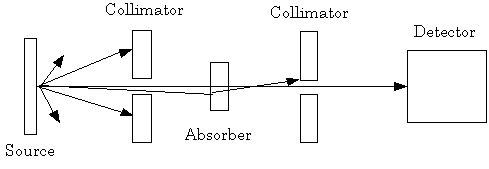
\includegraphics[width=0.7\linewidth]{images/GMAimage008.png}}
    \caption{A diagram of Gamma-ray Spectroscopy}
    \label{fig:GMAimage008}
\end{figure}

\section{References}
\label{sec:References}

\begin{enumerate}
    \item \href{http://www.webelements.com}{\textbf{Web Elements Period Table of Elements}}

    \item Segre, Emilio. ``\href{http://physics111.lib.berkeley.edu/Physics111/Reprints/GMA/Scattering\%20From\%20Center\%20appendix\%20a.pdf}{\textbf{Appendix A: Scattering from a Fixed Center of Force}}.'' \emph{Nuclei and Particles}, Second Edition, WA Benjamin Inc. London (1977).
    
    \item Yoshizawa, Yasukazu. ``\href{http://physics111.lib.berkeley.edu/Physics111/Reprints/GMA/betaandgammarayspecofCs137.pdf}{\textbf{Beta and Gamma Ray Spectroscopy of C 137,}}'' Nuclear Physics 5, 1958, pp. 122-140. \#QC770.N8
    
    \item Canberra Counter/Timer 1772 \href{http://physics111.lib.berkeley.edu/Physics111/Reprints/GMA/Canberra\_counter\_1772.pdf}{\textbf{Instruction Manual}}
    
    \item Equipment Manuals; \href{http://physics111.lib.berkeley.edu/Physics111/Equipment\_Manuals/GMA/indexequipGMA.html}{\textbf{GMA Equipment Manuals}}
    
    \item DG645 Digital Pulser  \href{http://physics111.lib.berkeley.edu/Physics111/Equipment_Manuals/GMA/DG645m.pdf}{\textbf{Manual}}
    
    \item R. D. Evans, \href{http://physics111.lib.berkeley.edu/Physics111/Reprints/R.D.Evans\%20Atomic\%20Nucleus/The\%20Atomic\%20Nucleus\%20Evans\%20full\%20text.pdf}{\textbf{The Atomic Nucleus}}. McGraw Hill (1972).
    
    \item RCA 6810A Photomultiplier Tube \href{http://physics111.lib.berkeley.edu/Physics111/Reprints/GMA/OCR\%20RCA\%206810A\%20photomultiplier\%20tube.pdf}{\textbf{PMT 6810}}
\end{enumerate}

\noindent Other reprints and reference materials can be found on the \href{http://physics111.lib.berkeley.edu/Physics111/Reprints/GMA/GMA\_index.html}{\textbf{Physics 111 Library Site}}

\end{document}
